%%%%%%%%%%%%%%%%%%%%%%%%%
% Baseline selection
%%%%%%%%%%%%%%%%%%%%%%%%%

The baseline selection for the razor boost analysis is driven by the two components of its name, in
addition to requiring the event to be of good quality.
As we use the razor variables, we need to be able to compute them. This means that there should be
at least two jets in the final state. The megajets from which the razor variables are computed, are
constructed from the AK5 jets (see Table~\ref{tab:object_jets} for their definition).  
After sensitivity studies, it was decided to raise the requirement on the jet multiplicity from two
to three, reducing the background, while maintaining very good signal efficiency. The signal
processes that are the main focus of this analysis usually have even more reconstructed jets, as
can be seen from Fig.~\ref{fig:njets_sig_BG}. In order to remain as inclusive as possible, we did
not, however, raise this threshold further.
The minimal requirements on the razor variables themselves are, as mentioned before, $\mr > 800\GeV$
and $\rsq > 0.08$.
This selection is complementary to that of previous razor analyses. By requiring a larger
minimal \mr, consistent with the boosted scenario, we can explore the low \rsq region, which is
important for signals with more compressed mass spectra.
Access to the boosted phase space is also provided by making the requirement that at least one AK5
jet satisfies $\pt > 200\GeV$.
In summary, events are required to satisfy the following baseline selection:
\begin{enumerate}
 \item Satisfy all cleanup filters, as listed in Section~\ref{sec:event_cleaning},
 \item Have at least one good primary vertex,
 \item Have at least three selected AK5 jets of which at least one has  $\pt > 200$\GeV, thereby
 defining the boosted phase space,
 \item $\mr > 800\GeV$ and $\rsq > 0.08$ (where the megajets are constructed from the selected AK5
jets).
\end{enumerate}
In addition to these requirements, we also impose the trigger conditions. 
For data events, we require that one of the triggers listed in Table~\ref{tab:boost_triggers} was
fired. 
For simulated events, we apply an event-by-event trigger efficiency, as explained in
Section~\ref{sec:boost_data_trigger}. 

\begin{figure}[htbp]
 \centering
 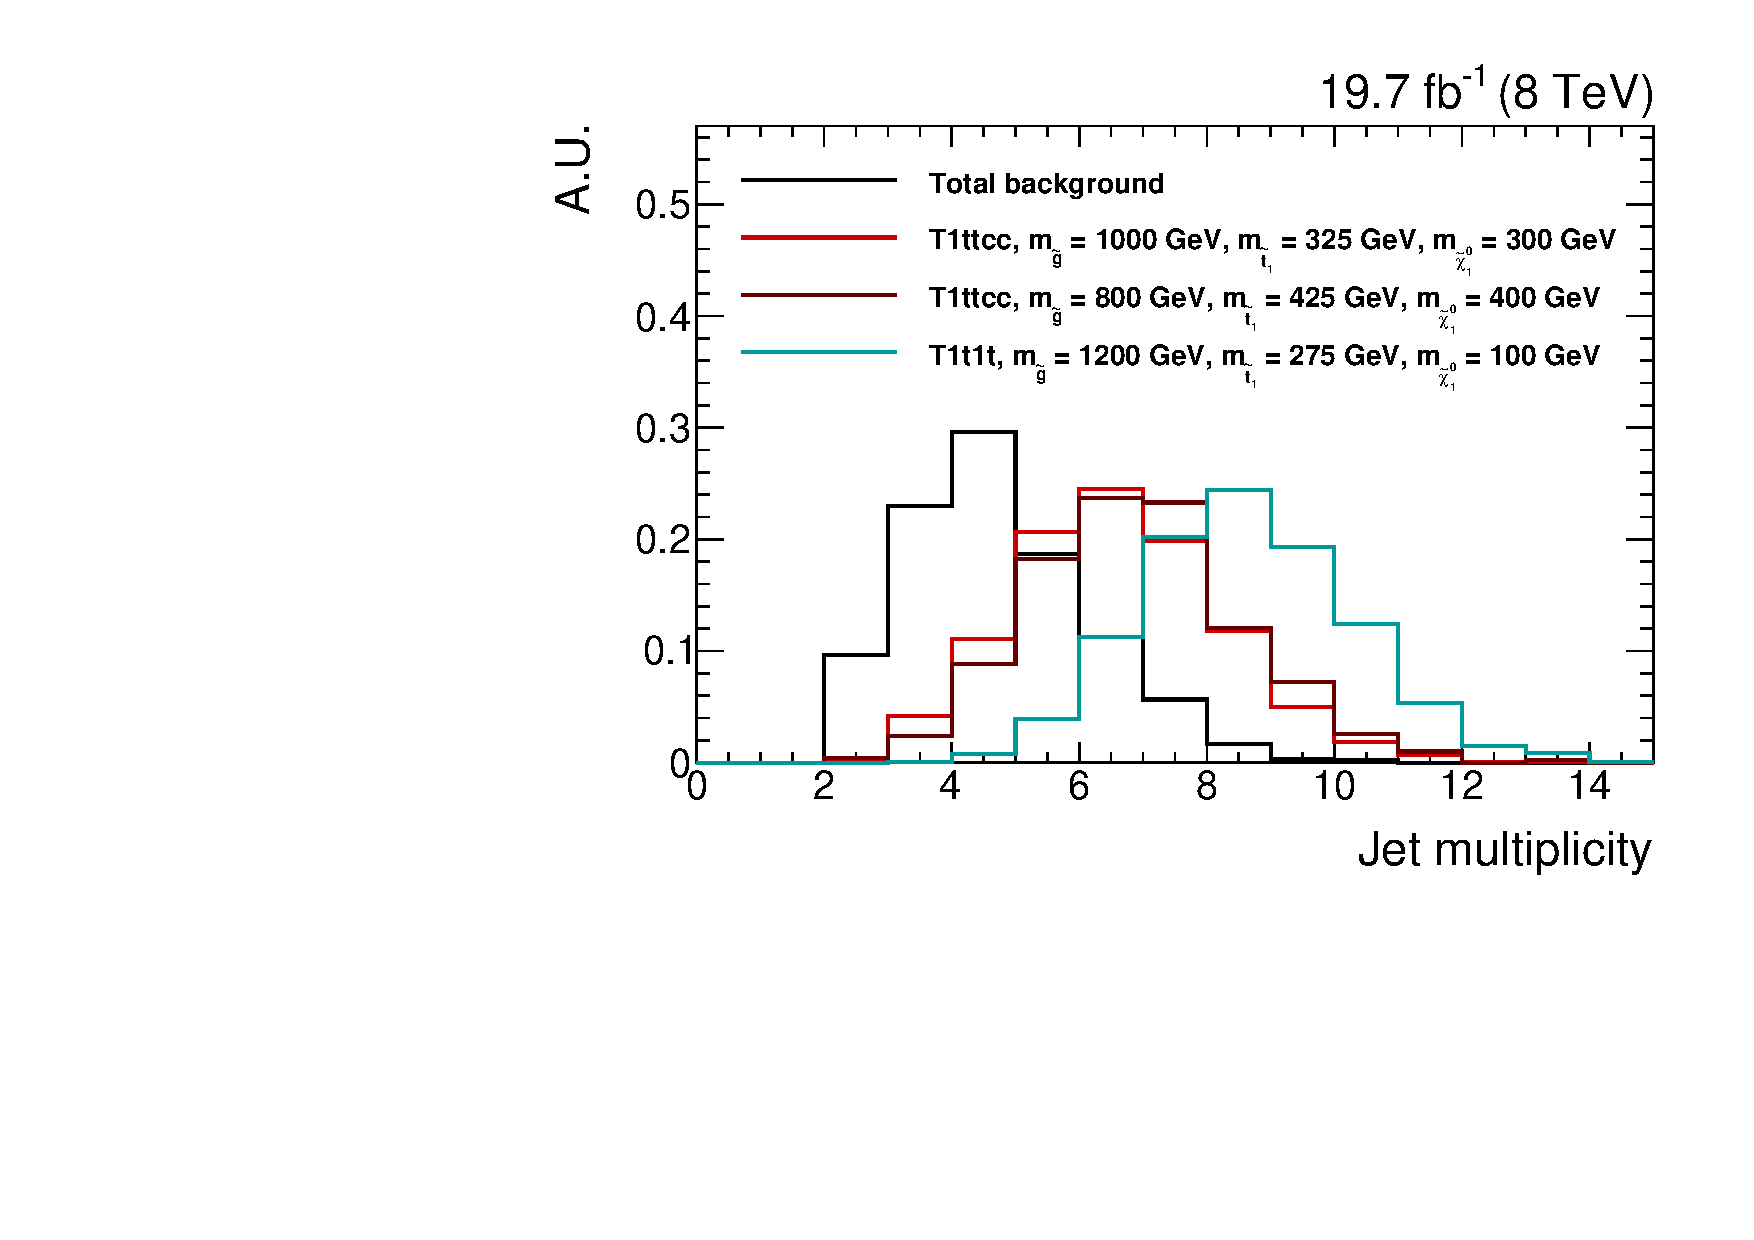
\includegraphics[width=0.6\textwidth]{figures/razor_selection/njets_signal_region}
 \caption{Distribution of the number of jets for the total SM background and three example signal
points in the signal region. The full selection except for the jet multiplicity requirement was
applied. The histograms are normalized to unit area.
 \label{fig:njets_sig_BG}}
\end{figure}

In Fig.~\ref{fig:boost_baseline_dataMC} we compare the observed data to the simulation for
events passing this baseline selection. 
As will be the case for all following comparisons of data versus simulation, the simulation is
scaled to the expected number of events according to the (NN)LO cross section of each process.
In addition, the simulated events are reweighted in order to correct for mismodelling of the
pileup, trigger, $\cPqb$ tagging, top \pt distribution, etcetera. Most of these reweightings are
performed for each region, but for some, such as the $\cPqb$ tagging scale factors, the reweighting
is only applied when the source of the reweighting is used explicitly in the selection. For the
$\cPqb$ tagging this would be a specific requirement or veto on the $\cPqb$-tagged jet
multiplicity. Hence, the reweighting is not applied in the baseline selection region. 
A full overview of these sources of event reweighting is given in
Table~\ref{tab:boost_reweighting}. Each of these sets of event weights has an associated
uncertainty. These will be taken into account as systematic uncertainties on the final background
prediction, as explained in more detail in Section~\ref{sec:boost_systematics}. 
From the figure, we see that there is good agreement between data and simulation for the highest
$\mr$ and $\rsq$ bins, \ie when the contribution of QCD multijet MC is very small. 
For the first $\mr$ and $\rsq$ bins, which are dominated by multijet production, the simulation
underpredicts the data by about 50\%. 

\begin{table}[htpb]
  \caption{Sources of event reweighting, when they are applied, and to which process. 
  \label{tab:boost_reweighting}}
  \begin{center}
  \begin{tabular}{l l l}
    \toprule
    Source & Region & Process \\
    \midrule
    Pileup & All & All \\
    Trigger & All & All \\
    $\cPqb$ tagging & If $\cPqb$ tagging used & All \\
    $\W$ tagging & If $\W$ tagging used & All \\
    Top \pt spectrum & All & $t\bar{t}$ \\
    Initial state radiation & All & Signal \\
    \bottomrule
  \end{tabular}
  \end{center}
\end{table}
 
The data/MC comparison is also displayed in table form. The first section of Table~\ref{tab:cutflow}
shows the expected number of events for the different background processes for several steps in the
baseline cutflow. The entry listed as ``No selection" corresponds to the total number of events
expected when no selection is applied. It is equal to the cross section of the process times the
integrated luminosity. 
The row corresponding to ``$n_{PV} > 0$'' gives the event counts after applying the
cleaning filters, the relevant event reweightings, and the requirement that there be at least one
good primary vertex.
The background composition after the full baseline selection, expressed in percentages, is reported
in Table~\ref{tab:BG_comp_percent}.  

\begin{figure}[htbp]
 \centering
 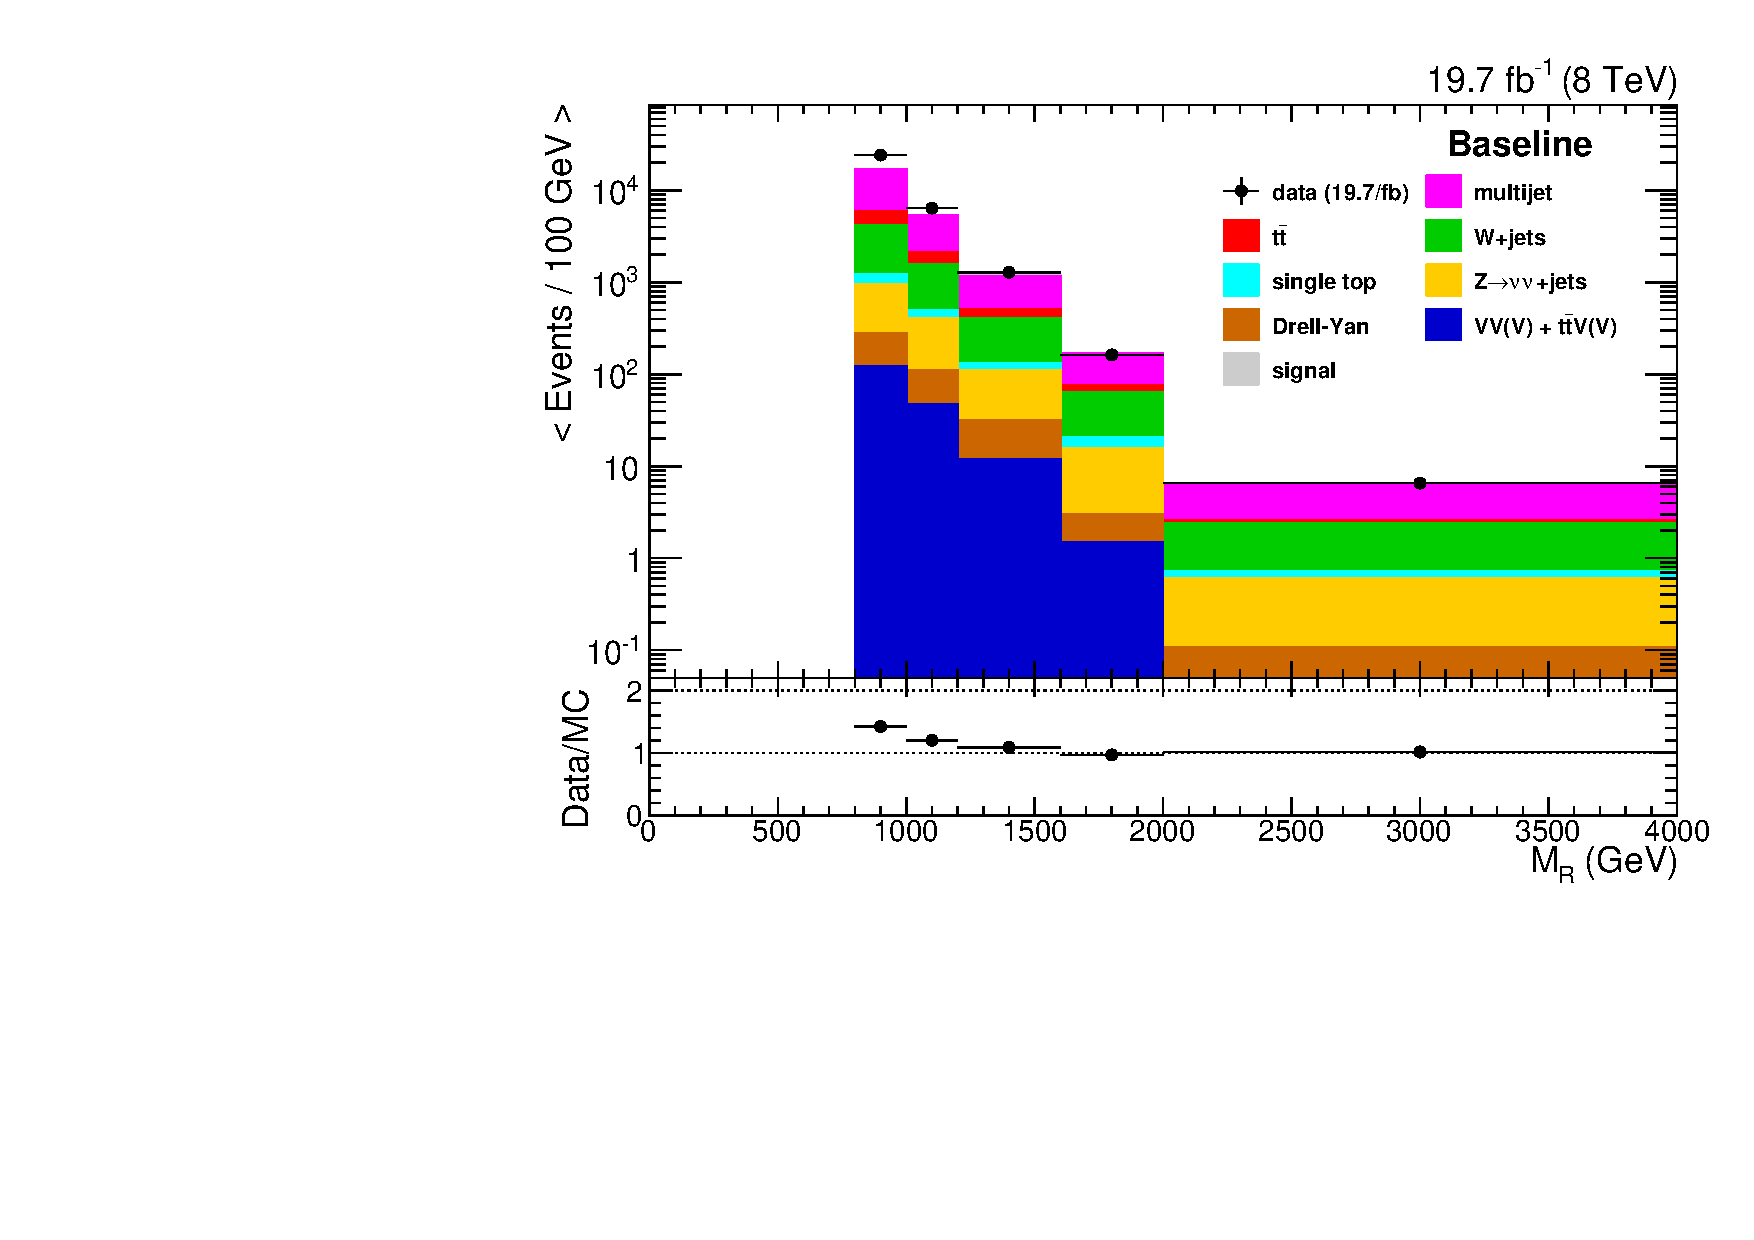
\includegraphics[width=0.48\textwidth]{figures/razor_selection/plots/DataMC_MR_HLT_width}
 ~
 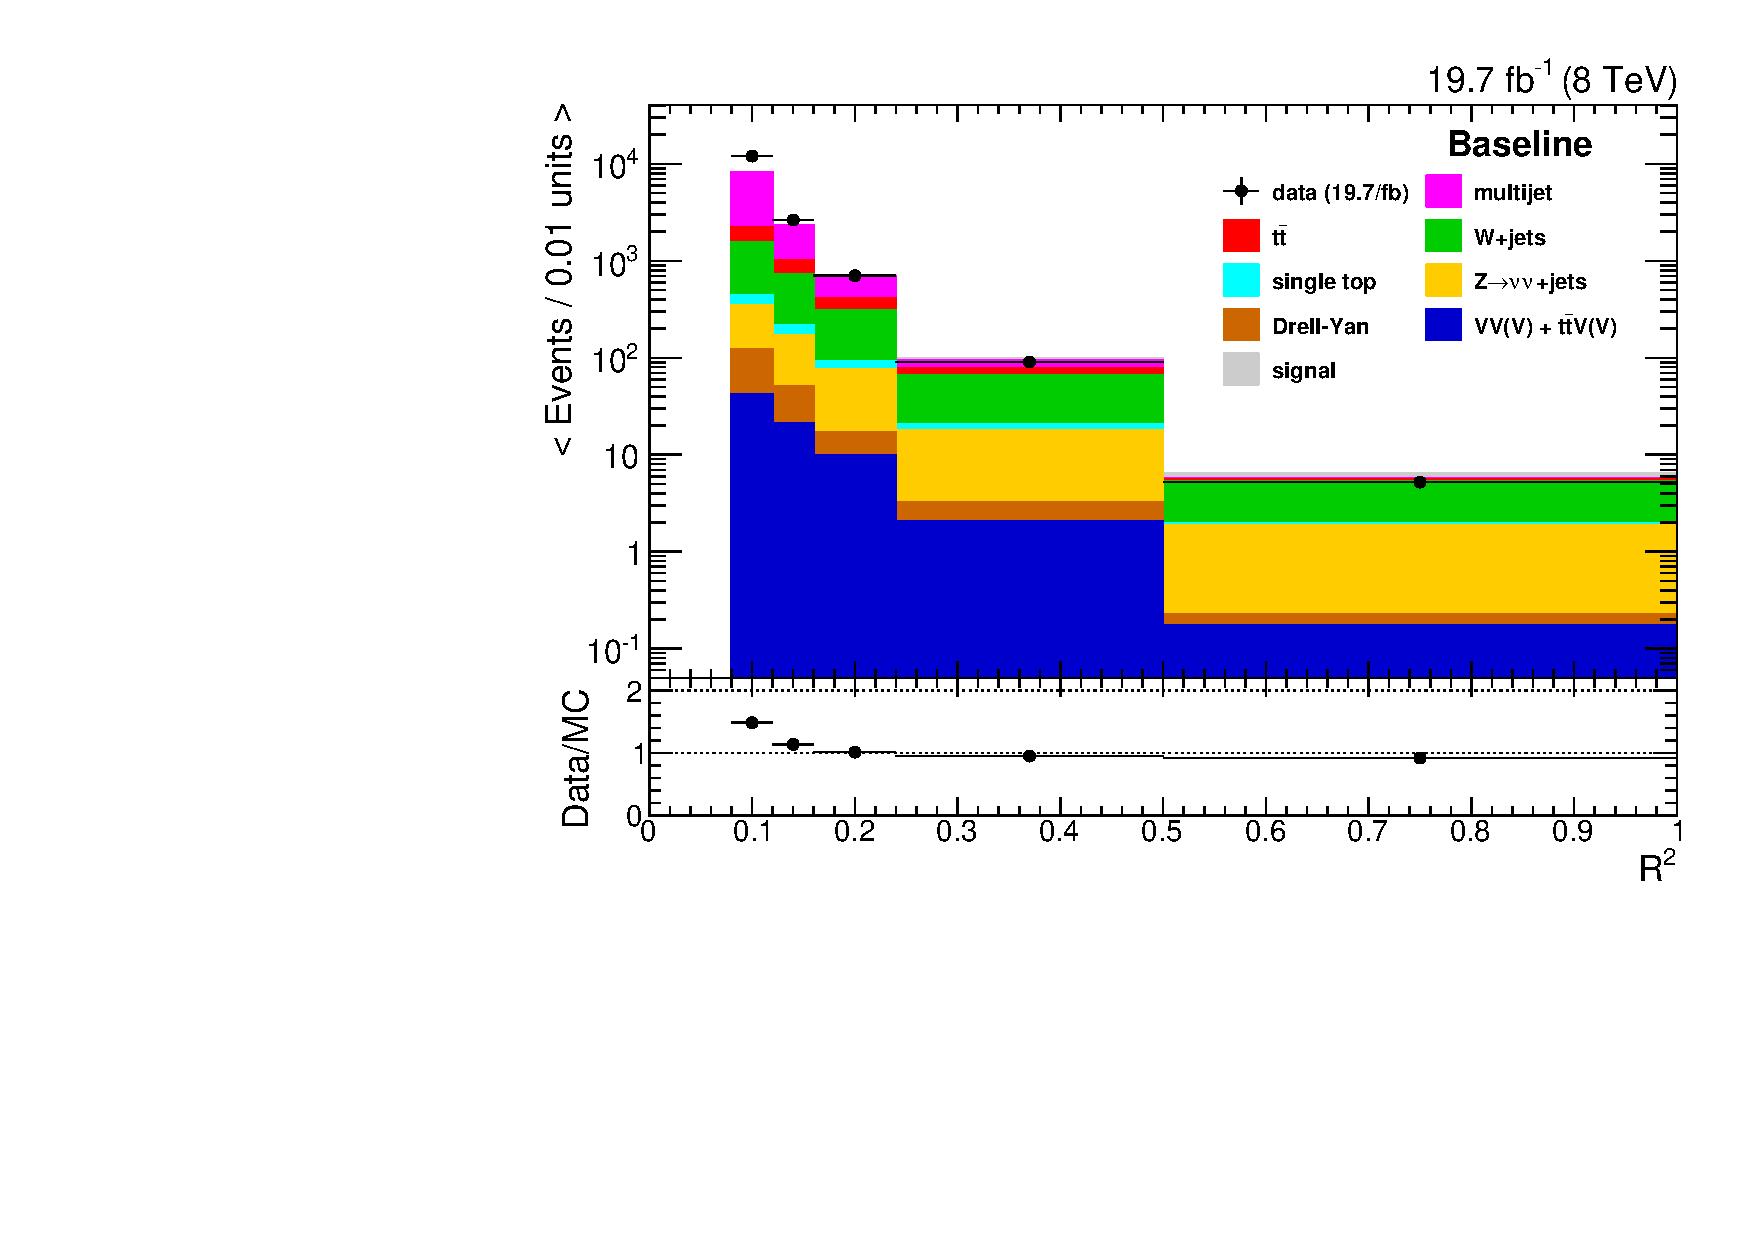
\includegraphics[width=0.48\textwidth]{figures/razor_selection/plots/DataMC_R2_HLT_width}
 \caption{Comparison between data and simulation for the $\mr$ (left) and $\rsq$ (right)
distribution in the baseline selection region. The bin entries are scaled proportional to the bin
width.
 \label{fig:boost_baseline_dataMC}}
\end{figure}
